% Options here are passed to the article class.
% Most common options: 10pt, 11pt, 12pt
\documentclass[10pt]{datasheet}

% Input encoding and typographical rules for English language
\usepackage[utf8]{inputenc}
\usepackage[english]{babel}
\usepackage[english]{isodate}

% tikz is used to draw images in this example, but you can
% also use \includegraphics{}.
\usepackage{graphicx}

% These define global texts that are used in headers and titles.
\title{EC02: Small Decimal Encoder}
\author{Andrews54757}
\tags{encoders, decimal}
\date{December 2022}
\revision{Revision 1}
\begin{document}
\maketitle

\section{Features}

\begin{itemize}
\item{Small and simple stacked design with demibolts.}
\item{Encodes up to 1000 item types.}
\item{Uses up to four carts for 1 code/56 gt throughput}
\end{itemize}

\section{Applications}

\begin{itemize}
\item{Encoding items}
\end{itemize}

\section{General Description}
The EC02 small item to decimal encoder uses demibolts and a simple layered design. It can handle up to 1000 item types.

% Switch to next column
\vfill\break

\begin{figure}[h]
    \centering
    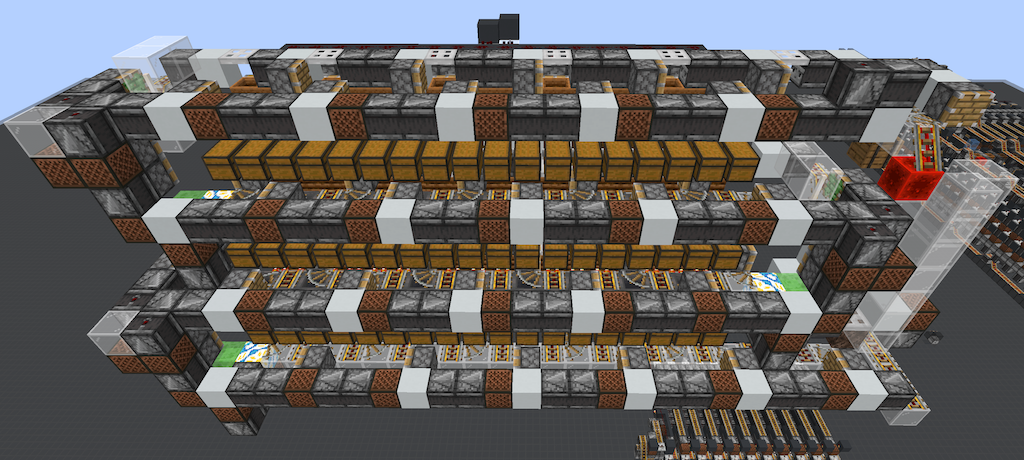
\includegraphics[width=0.48\textwidth]{small.png}
    \caption{\centering Small Decimal Item Encoder}
\end{figure}

% For wide tables, a single column layout is better. It can be switched
% page-by-page.
\onecolumn

\section{Device Specifications}

\begin{table}[h]
    \caption{Inputs}
    \begin{tabularx}{\textwidth}{l | c | X}
        \thickhline
        \textbf{Name} & \textbf{Range} & \textbf{Description} \\
        \hline
        Item input & Item & Item for encoding. \\
        \thickhline
\end{tabularx}
\end{table}

\begin{table}[h]
    \caption{Outputs}
    \begin{tabularx}{\textwidth}{l | c | X}
        \thickhline
        \textbf{Name} & \textbf{Range} & \textbf{Description} \\
        \hline
        Item output & Item & Outputs the inputted item. \\
        \hline
        Item Code 1 & 6-15 & First digit of code. \\
        Item Code 2 & 6-15 & Second digit of code. \\
        Item Code 3 & 6-15 & Third digit of code. \\
        \thickhline
\end{tabularx}
\end{table}

\begin{table}[h]
    \caption{Device Specifications}
    \begin{tabularx}{\textwidth}{l | c c c | c | X}
        \thickhline
        \textbf{Parameter} & \textbf{Min.} & \textbf{Typ.} & \textbf{Max.} &
        \textbf{Unit} & \textbf{Conditions} \\
        \hline
        Throughput  & 56 & - & - & gt & Normal Usage \\
        \hline
        Active Lag & +0.5 & +1 & +2 & ms & At fullspeed. Ryzen 5 3600, 2GB RAM. MC 1.18.1 with Lithium. \\
        \hline
        MC Version & 1.16 & 1.17.1 & - & MCV & Latest version at time of writing: 1.19.3\\
        \hline
        Dimensions & & 28 x 13 x 17 & & Blocks & \\
        \thickhline
\end{tabularx}
\end{table}
\newpage
\section{Testing Data}
\begin{table}[h]
\caption{Executed Tests}
\begin{tabularx}{\textwidth}{l | X}
    \thickhline
    \textbf{Test} & \textbf{Result} \\
    \hline
    Item encoding test & Device was able to encode with item input \\
    \hline
    Throughput test & Device was able to encode at 8gt throughput with randomized input. \\
    \thickhline
\end{tabularx}
\end{table}

\section{Download Information}
\begin{table}[h]
    \caption{Download Information}
    \begin{tabularx}{\textwidth}{l | l | l | X}
        \thickhline
        \textbf{Identifier} & \textbf{MC} & \textbf{File} & \textbf{Description} \\
        \hline
        EC01 & 1.17.1 & \href{https://github.com/Soontech-Annals/Archive/blob/8413f90a054b6c415703bae02badeba7541344f6/Archive/encoders/EC02\%20Small\%20Decimal\%20Encoder/EC02\_small\_decimal\_encoder.litematic?raw=1}{EC02\_small\_decimal\_encoder.litematic} & Schematic of encoder. \\
        \hline
        \thickhline
    \end{tabularx}
\end{table}

\end{document}

